% =====================================================================
% Morning60s — C&C 2026 Poster Submission (single-column, ANONYMIZED)
% =====================================================================
\documentclass[manuscript,anonymous,review]{acmart}

\setcopyright{none}
\acmConference[C\&C '26]{ACM Creativity \& Cognition 2026}{June 2026}{London, UK}
\acmBooktitle{ACM Creativity \& Cognition 2026 (C\&C '26), June 2026, London, UK}
\settopmatter{printacmref=false, printccs=false, printfolios=true}

\usepackage{graphicx}
\usepackage{float}
\usepackage{microtype}
\usepackage{hyperref}
\usepackage{fancyhdr}

\title{Morning60s: Get Out of Bed in 60 Seconds}

\author{}
\affiliation{%
  \institution{}
  \country{}
}
\email{}
\renewcommand{\shortauthors}{}

\begin{document}

% acmart uses a custom page style called "standardpagestyle";
% overriding just "plain" / "fancy" is not enough---we must override that one too.
\fancypagestyle{standardpagestyle}{%
  \fancyhf{}%
  \fancyfoot[C]{\thepage}%
  \renewcommand{\headrulewidth}{0pt}%
  \renewcommand{\footrulewidth}{0pt}%
}
\fancypagestyle{plain}{%
  \fancyhf{}%
  \fancyfoot[C]{\thepage}%
  \renewcommand{\headrulewidth}{0pt}%
  \renewcommand{\footrulewidth}{0pt}%
}
\pagestyle{standardpagestyle}

% Kill the "2026. Manuscript submitted to ACM" first-page footnote
% that acmart's manuscript mode prints above the copyright strip.
\makeatletter
\renewcommand{\@manuscriptdates}{}
\renewcommand{\@copyrightpermission}{}
\makeatother

\begin{abstract}
Morning60s is an app that helps users get out of bed within 60 seconds by providing immediate rewards. If users get out of bed within 60 seconds, they collect a ``cyber breakfast'' sticker from a library of over 100 geometric-style designs. Users are also encouraged to write a plan or intention for the next morning the day before, as a form of motivation. To prevent cheating-in-bed, Morning60s integrates the Qwen-VL vision model and requires users to take a photo of themselves standing on the ground as verification.
\end{abstract}

\keywords{Wake-up; 60 seconds; cyber breakfast; sticker collection; night-before intention; Qwen-VL; anti-cheating; behavior change.}

\maketitle

% Teaser figure: upload `teaser.png` to the Overleaf project root,
% then remove the `%` at the start of each line and Recompile.
%\begin{figure}[t]
%  \centering
%  \includegraphics[width=\linewidth]{teaser.png}
%  \caption{Morning60s: start $\rightarrow$ 60s countdown $\rightarrow$ proof photo $\rightarrow$ cyber breakfast sticker $\rightarrow$ calendar stamp.}
%  \label{fig:teaser}
%\end{figure}

\section{Problem}
Many people struggle to get out of bed and often check social media immediately after waking up, which can lead to wasted time and negative emotions. At the start of the day, many people even spend more than one hour staying in bed before getting up.

\section{Research question}
We take this everyday failure as a design-research question:

\begin{quote}
\emph{Can a 60-second, photo-verified micro-ritual---built around a collectible illustrated reward and a user-written intention from the night before---help people reliably get out of bed, and reframe the first minute of the day as a small creative act rather than a chore?}
\end{quote}

Concretely, we ask: (i) what kind of \emph{reward} is appealing enough to compete with the pull of social media in bed, and (ii) what kind of \emph{verification} is strict enough to keep that reward honest without feeling punishing. Morning60s is our first attempt at an answer.

\section{Morning60s}
Morning60s is an app that helps users get out of bed within 60 seconds by providing immediate rewards. The design is built around three ideas: an \emph{immediate reward} right after getting up, a \emph{night-before intention} that gives the morning a reason, and a \emph{vision-based proof photo} that makes the whole system honest.

\subsection{Immediate reward: cyber breakfast}
If users get out of bed within 60 seconds, they collect a ``cyber breakfast'' sticker from a library of over 100 geometric-style designs (Figure~\ref{fig:cyber-breakfast}). The sticker is revealed on a reward card---the design of the card itself is part of the appeal---and added to a personal collection screen the user can browse later.

\begin{figure}[!htbp]
  \centering
  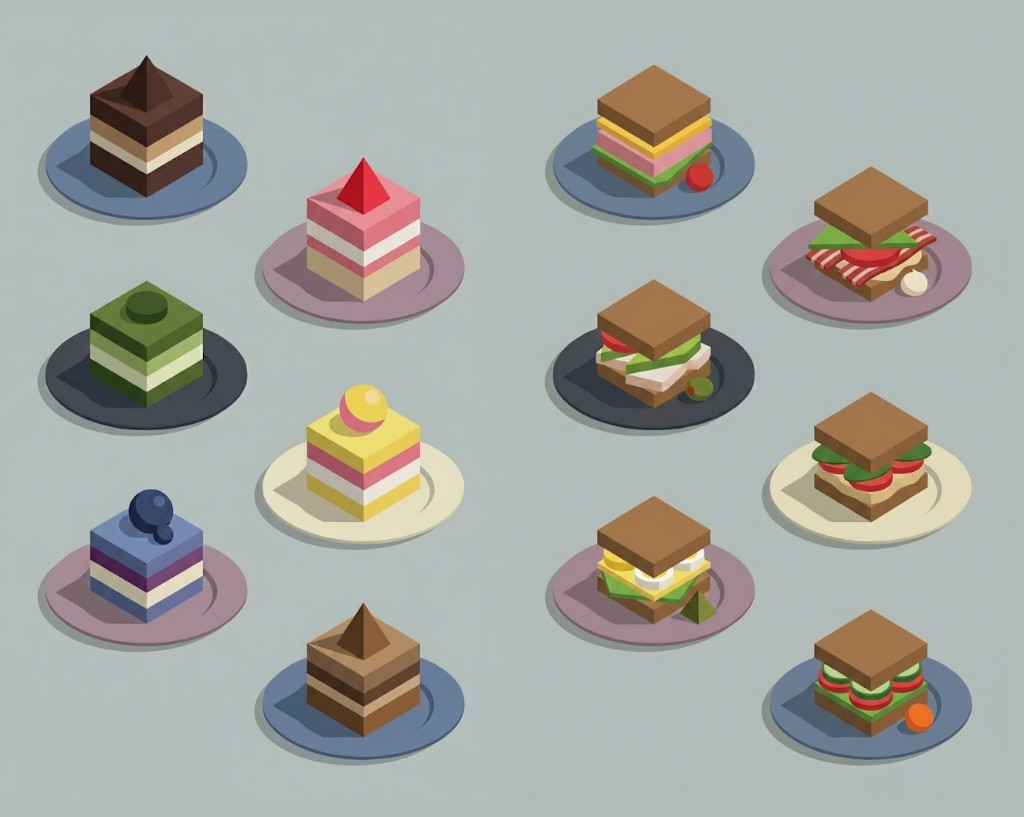
\includegraphics[width=0.85\linewidth]{cyber_breakfast.png}
  \caption{A sample of the ``cyber breakfast'' sticker library: isometric, geometric-style illustrations of breakfast items (layered cakes, sandwiches, etc.) used as the immediate reward after a successful 60-second wake-up.}
  \label{fig:cyber-breakfast}
\end{figure}

We call these stickers ``cyber breakfast'' on purpose. The first minute of the day is usually the opposite of eating breakfast: people reach for the phone and scroll in bed. Morning60s replaces that first reach-for-the-phone moment with a small, playful object that only unlocks if the user has \emph{already} stood up. The stickers are geometric, illustrative, slightly absurd (fried eggs, toast, coffee cups drawn as flat shapes). Because the library has more than 100 designs and a new one is drawn each morning, the collection itself becomes a reason to get up again tomorrow. This is the creativity angle of the app: the reward is not a number, a streak, or a badge---it is a small piece of illustration you earn by being out of bed.

\subsection{Night-before intention}
Users are encouraged to write a plan or intention for the next morning the day before (for example, \emph{going for a run} or \emph{cooking a nice meal}), which serves as a form of motivation. The intention is entered on an evening screen the night before and surfaced the next morning right next to the 60-second challenge.

The design is inspired by a very ordinary observation. As children, on the morning of a school outing, we could jump out of bed at the first alarm. As adults, on the morning of a trip, we wake up just as easily---sometimes before the alarm even rings. The hard part of getting up has never really been the body; it is that on an ordinary morning there is nothing to look \emph{forward} to. Morning60s tries to recreate that feeling on a regular Tuesday by asking users to \emph{collect a desire} the night before: a small, concrete thing they actually want to do tomorrow morning. That desire, written in the user's own words the evening before, is what the 60-second challenge is in service of. This is our answer to a common failure mode of alarm apps: when the alarm rings, the user has no reason to get up, only a reason to dismiss the alarm.

\subsection{Anti-cheating: Qwen-VL verification}
Morning60s includes an anti-cheating mechanism: we integrate the Qwen-VL vision model and require users to take a photo of themselves standing on the ground as verification. This prevents users from earning rewards while staying in bed.

Concretely, after the 60 seconds the app opens the camera and asks for a quick selfie-style photo that must show the user's legs and the floor. The image is sent to the vision model, which returns a pass/fail judgment; only a pass unlocks the sticker. Without this check, any reward system is just a button the user can press while still under the covers. The photo is what makes the contract between user and app real.

\section{A morning with Morning60s}
A full wake-up flow is intentionally short.
\begin{enumerate}
  \item The app opens to a warm, daylight-themed wake screen and shows the intention the user wrote the night before.
  \item The user taps \emph{Start}; a 60-second countdown begins. The screen stays readable in a low-brightness, just-woke-up state.
  \item When the user stands up, they tap \emph{I'm up}. The camera opens and the user takes a proof photo showing their legs and the floor.
  \item Qwen-VL verifies the photo. On a pass, a reward card flips over and reveals today's cyber-breakfast sticker.
  \item The day's box on a streak calendar gets stamped. The user can come back later to browse the full sticker collection and the calendar.
\end{enumerate}
The whole flow, from waking up to stamped calendar, is a single minute of interaction plus a few seconds of camera and verification. Everything else in the app---the evening intention screen, the calendar, the collection, the day-recap and night-recap views---exists to frame that one minute and make it feel meaningful.

\section{Why it is different}
There are many alarm and sleep-tracking apps on the market, but they usually focus on improving sleep quality, tracking sleep patterns, or optimizing bedtime routines. Morning60s, however, focuses on a single, clearly defined scenario: \textbf{the short period each morning between waking up and getting out of bed}. It addresses a smaller and more concrete problem---helping users get out of bed immediately. While this is a very focused problem, it is also a common and frustrating pain point for many people in the age of social media.

We also differ from existing alarm apps in \emph{how} we motivate action. Instead of punishment (louder alarms, CAPTCHAs, shake-to-stop, pay-if-you-fail), Morning60s uses a collectible, illustrative reward plus a user-written intention. The proof photo is not there to punish; it exists so the reward stays earned.

\section{Prototype}
An initial iOS version (SwiftUI) with all core features is working:
\begin{itemize}
  \item The 60-second challenge with countdown and \emph{I'm up} button.
  \item Cyber-breakfast reward cards, drawn from a growing illustrated library.
  \item A night-before intention entry on the evening screen.
  \item Qwen-VL photo verification via a thin backend service, with a retry path if the photo does not pass.
  \item A streak calendar that places an animated stamp on each completed day and a collection view for earned stickers.
  \item A time-aware \emph{Today} tab that automatically shows the wake screen in the morning, a day-recap in the afternoon, and a night-recap---including the intention entry---in the evening (Figure~\ref{fig:recap}).
\end{itemize}

\begin{figure}[!htbp]
  \centering
  \begin{minipage}[t]{0.4\linewidth}
    \centering
    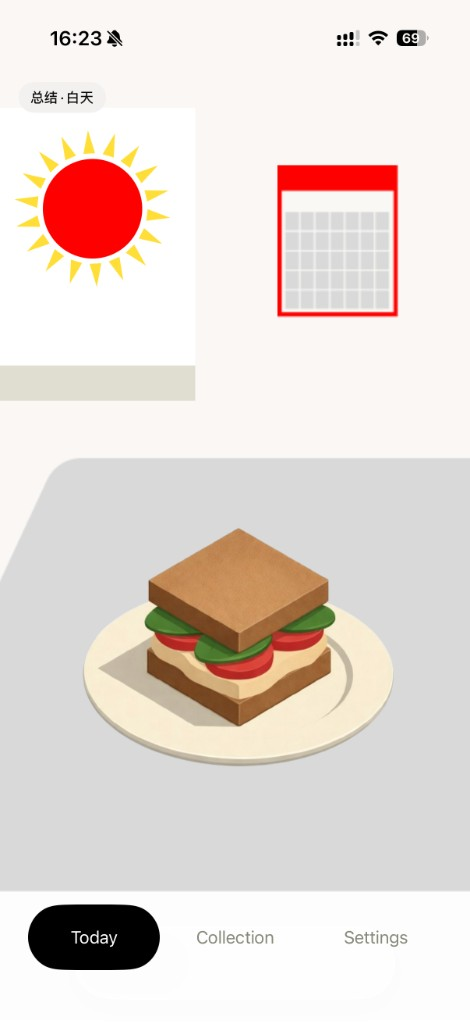
\includegraphics[width=\linewidth]{recap_day.png}
  \end{minipage}\hfill
  \begin{minipage}[t]{0.4\linewidth}
    \centering
    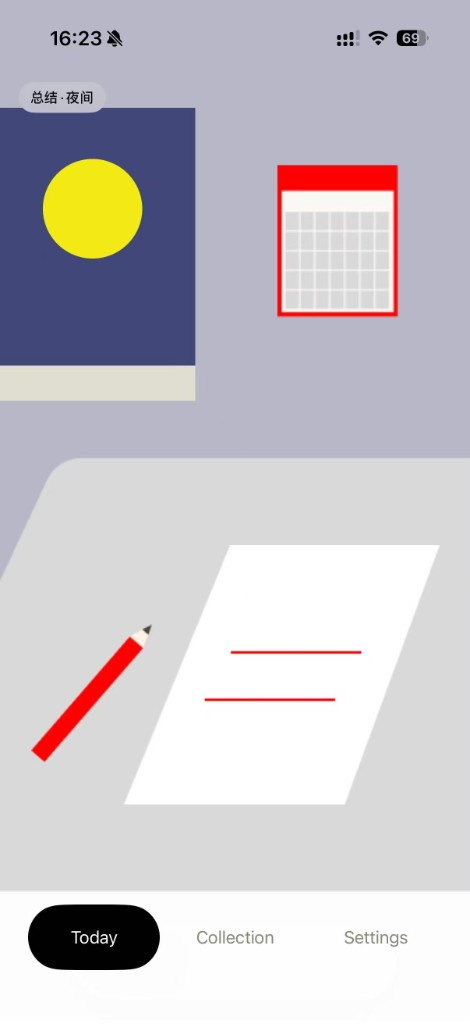
\includegraphics[width=\linewidth]{recap_night.png}
  \end{minipage}
  \caption{The time-aware \emph{Today} tab. Left: day recap (afternoon), featuring the daily cyber-breakfast sticker and a calendar card. Right: night recap (evening), where the pencil-and-paper card invites the user to write a night-before intention. The tab switches automatically based on the system clock, so the app frames the user's \emph{whole day} around the one-minute wake-up moment rather than only the alarm.}
  \label{fig:recap}
\end{figure}

\section{Ethics and privacy}
Morning60s asks the user for a daily proof photo. A privacy-first deployment should minimize retention, avoid storing images by default, clearly communicate what is transmitted and why, and support on-device verification when feasible.

\section{Contribution to Creativity \& Cognition}
We see three contributions to the C\&C research community.

\textbf{A new design target for creativity research: the waking-up window.} Work on behavior-change apps usually targets either long timescales (sleep, habits, streaks over weeks) or the moment of the alarm. We isolate a different unit: \emph{the short period each morning between waking up and getting out of bed}. Morning60s is a concrete design artifact showing this window is expressive enough to host a creative micro-ritual, not just a louder alarm.

\textbf{Creativity-as-reward, not punishment-as-coercion.} Most wake-up apps coerce action through escalation (louder alarms, CAPTCHAs, monetary penalties). Morning60s replaces that with a collectible, illustrated ``cyber breakfast'' sticker drawn from a library of over 100 geometric-style designs, plus a night-before intention written in the user's own words. This is a design pattern the C\&C community can inspect, critique, and reuse: the reward itself is a small creative object, and the creativity lives on both sides---in the illustration library we author, and in the intention the user writes.

\textbf{Vision-language models as honesty scaffolds for creative reward systems.} A creative reward only works if it is earned. We use Qwen-VL not to generate content but as a lightweight verifier that the user is standing on the floor. This positions vision-language models in a role the C\&C community has discussed less than generation: a low-friction ``referee'' that keeps playful, collectible reward systems from collapsing into dishonest self-report. Morning60s is an early case study of this pattern, and of the ethical and privacy trade-offs it forces designers to confront.

Together, these contributions offer the C\&C community a small, self-contained example of how creative design, everyday behavior, and AI-based verification can be composed into a single one-minute ritual.

\section{Conclusion}
Morning60s treats the first 60 seconds of the day as a small, verifiable, rewarding ritual: a 60-second challenge, a cyber-breakfast sticker from a library of over 100 geometric-style designs, a night-before intention, and a vision-model check that prevents cheating in bed. It is not another alarm or sleep-tracker. It targets the short period between waking up and getting out of bed---a concrete, common pain point in the age of social media.

\end{document}
